\documentclass{beamer}
\usetheme{Madrid} % You can change the theme (e.g., "Berlin", "Copenhagen", "Frankfurt")



% Title, Author, and Date
\title[Mellin Transform]{Mellin Transform}
\author[]{Mohammad Mahdi Elyasi}
\institute[Amirkabir University of Techonology]{
    Supervisor: Dr. Moradi \\[1cm] % Professor's Name
    Faculty of Electrical Engineering \\ % Faculty Name
}
\date{\today} % Automatically uses today's date


% Customize the title slide layout
\setbeamertemplate{title page}{
    % Blue strip (Madrid theme)
    \vspace*{-0.5cm} % Adjust vertical spacing
    \begin{beamercolorbox}[wd=\paperwidth,ht=0.4cm,dp=0.2cm,center]{frametitle}
    \end{beamercolorbox}

    % Logo below the strip
    \vspace{0.5cm}
    \centering
    
\includegraphics[width=0.2\textwidth]{amirkabir.png} % Replace with your logo file

    % Title details
    \vspace{0.5cm}
    {\usebeamerfont{title}\inserttitle\par}
    \vspace{0.3cm}
    {\usebeamerfont{author}\insertauthor\par}
    {\usebeamerfont{institute}\insertinstitute\par}
    \vspace{0.3cm}
    {\usebeamerfont{date}\insertdate\par}
}
% Begin Document
\begin{document}


% Title Slide
\begin{frame}
    
    \titlepage
\end{frame}

% Table of Contents Slide
\begin{frame}{Table of Contents}
    \tableofcontents
\end{frame}

% Section 1: Introduction
\section{Introduction}
\begin{frame}{Introduction}
    \begin{itemize}
        \item Brief introduction to Mellin Transform.
        \item Applications in mathematical analysis.
        \item Why mellin transform?
    \end{itemize}
\end{frame}

% Section 2: Mathematical Background
\section{Mathematical Background}
\begin{frame}{Mathematical Background}
    \begin{itemize}
        \item Key mathematical definitions.
        \item Important integral formulas.
        \begin{equation}
            \mathcal{M}\{f(x)\}(s) = \int_{0}^{\infty} x^{s-1} f(x) \, dx
        \end{equation}
        \begin{equation}
            \Gamma(s) = \int_{0}^{\infty} x^{s-1} e^{-x} \, dx
        \end{equation}
        
    \end{itemize}
\end{frame}


\subsection{Property Proof}
\begin{frame}{Property Proof}
    \begin{itemize}
        \item Linearity of Mellin Transform.
        \item Scaling properties.
        \begin{equation}
            \mathcal{M}\{x^a f(x)\}(s) = \mathcal{M}\{f(x)\}(s + a).
        \end{equation}
        \begin{equation}
            \mathcal{M}\{f(ax)\}(s) = a^{-s} \mathcal{M}\{f(x)\}(s).
        \end{equation}
    \end{itemize}
\end{frame}

\subsection{Examples}
\begin{frame}{Examples}
    \begin{itemize}
        \item Examples.
        \vfill % Push the image to the bottom
        \centering
        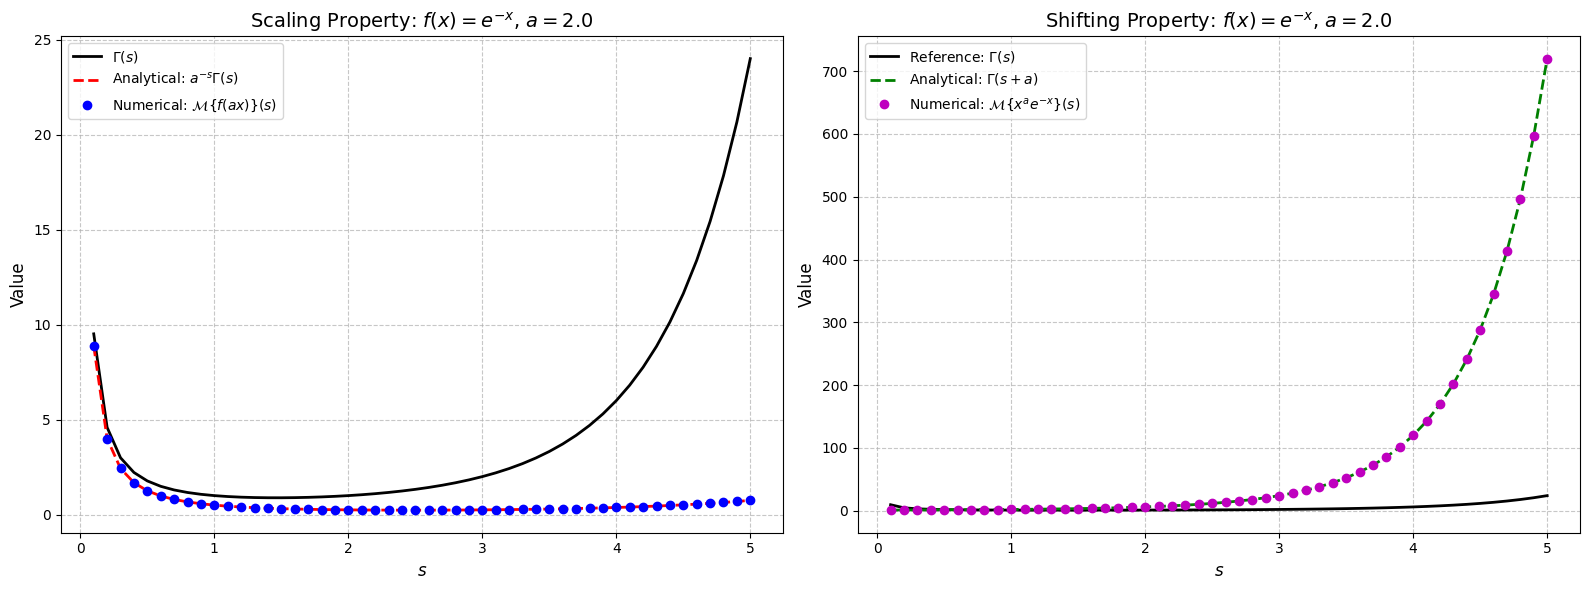
\includegraphics[width=0.8\textwidth]{Shifting and scaling.png} % Replace with your image file
        \\[0.2cm] % Add vertical spacing between image and caption
        {\small \textbf {Figure 1:}Shifting and Scaling Plots} % Caption text
    \end{itemize}
\end{frame}

% Section 3: Gamma and Mellin Transform Relations
\section{Gamma and Mellin Transform Relations}
\begin{frame}{Gamma and Mellin Transform Relations}
    \begin{itemize}
        \item Connection between Gamma functions and Mellin Transform.
        \item Relation of arithmetic number factorial and gamma function.\\[0.2cm]
        {\small \textbf if \( f(x) = e^{-x} \):}
        \begin{equation}
            \mathcal{M}\{e^{-x}\}(s) = \int_{0}^{\infty} x^{s-1} e^{-x} \, dx = \Gamma(s).
        \end{equation}
        \begin{equation}
            n! = \Gamma(n+1)
        \end{equation}
    \end{itemize}
\end{frame}

% Section 4: Case Study Result
\section{Case Study Result}
\begin{frame}{Case Study Result}
    \begin{itemize}
        \item Description of the case study.\\[0.2cm]
        \begin{equation}
            r^2 \phi_{rr} + r \phi_r + \phi_{\theta\theta} = 0
        \end{equation}
        \begin{align}
            \phi(r, \alpha) &= f(r), \quad \phi(r, -\alpha) = g(r), \quad 0 \leq r < \infty, \\
            \phi(r, \theta) &\to 0 \quad \text{as} \quad r \to \infty \quad \text{for all} \quad \theta \in (-\alpha, \alpha).
        \end{align}
        \vfill % Push the image to the bottom
        \centering
        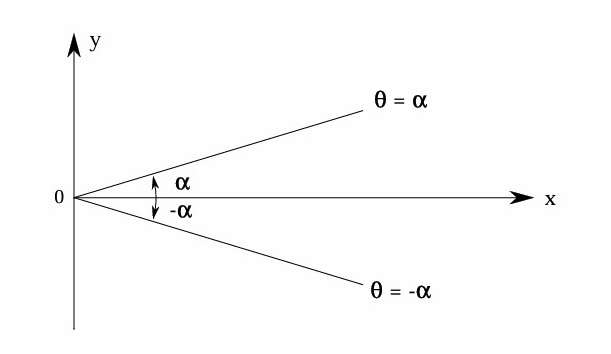
\includegraphics[width=0.8\textwidth,height=0.35\textheight]{infinite_wedge.jpg} % Replace with your image file
        \\[0.2cm] % Add vertical spacing between image and caption
        {\small \textbf {Figure 2:}Infinite Wedge} % Caption text
    \end{itemize}
\end{frame}

\subsection{Plot}
\begin{frame}{Plot}
    \begin{itemize}
        \item Plot for phi in designated variables.
        \vfill % Push the image to the bottom
        \centering
        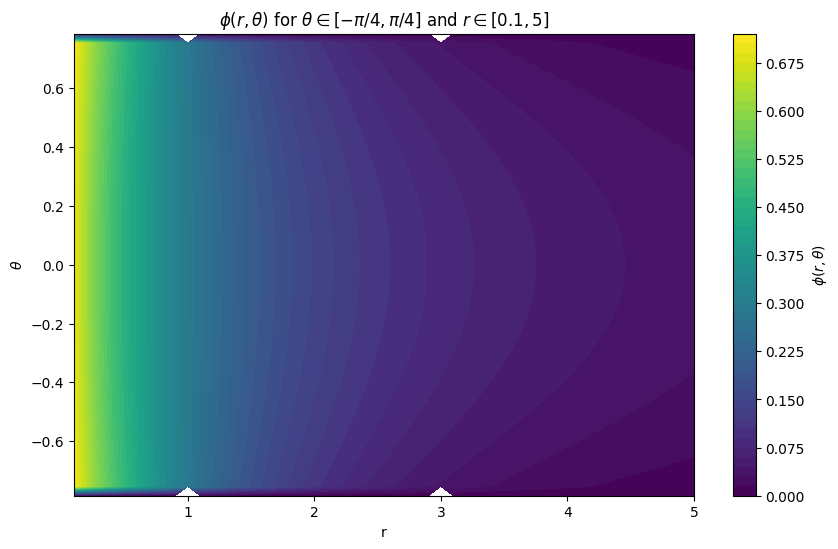
\includegraphics[width=0.8\textwidth]{Phi.png} % Replace with your image file
        \\[0.2cm] % Add vertical spacing between image and caption
        {\small \textbf {Figure 3:}Phi plot} % Caption text
    \end{itemize}
\end{frame}

% Section 5: Conclusion
\section{Conclusion}
\begin{frame}{Conclusion}
    \begin{itemize}
        \item Summary of key takeaways.
    \end{itemize}
\end{frame}

% Section 6: References
\section{References}
\begin{frame}{References}
    \begin{itemize}
        \item Debnath, Lokenath, and Dambaru Bhatta.\textit{l Transforms and Their Applications. 2nd ed.},CRC Press, 1995.
        \item  Github link,\textit{Mellin-transform} at \url{https://github.com/MohammadMahdiElyasi/Mellin-transform}.
    \end{itemize}
\end{frame}

% Section 7: Outro
\begin{frame}{Outro}
    \centering
    {\Large \textbf{Thank you for your attention!}} \vspace{1cm} % Ensures proper centering
    \vfill % Pushes the logo to the bottom
    
\includegraphics[width=0.2\textwidth]{amirkabir.png} % Replace with your logo file
\end{frame}

\end{document}
